\section{Results}
\label{sec:results}

\subsection{RQ1: Active-Learning Performance}

Table~\ref{tab:al-final} reports final-round results at 700 training labels. The
complete explanation-guided policy obtained the highest mean ROC--AUC
($0.9749\pm0.0040$) and AP ($0.9442\pm0.0057$). Uncertainty sampling reached
$0.9691\pm0.0046$ AUC, while random selection reached
$0.9634\pm0.0063$. Thus, the mean final AUC differences were 0.0058 relative to
uncertainty and 0.0115 relative to random.

\begin{table*}[t]
\centering
\caption{Final active-learning results at an equal budget of 700 training labels. Values are mean $\pm$ sample SD over five paired seeds. The 400 validation labels are additional.}
\label{tab:al-final}
\small
\begin{tabular}{lcccc}
\toprule
Strategy & ROC--AUC & AP & FPR (\%) & TPR (\%) \\
\midrule
Random & $0.9634\pm0.0063$ & $0.9194\pm0.0115$ & $21.73\pm4.59$ & $93.80\pm2.28$ \\
Uncertainty & $0.9691\pm0.0046$ & $0.9363\pm0.0076$ & $19.87\pm4.65$ & $95.60\pm1.14$ \\
$U+H$ & $0.9676\pm0.0031$ & $0.9371\pm0.0015$ & $17.20\pm5.15$ & $93.00\pm2.35$ \\
$U+V$ & $0.9692\pm0.0062$ & $0.9392\pm0.0073$ & $28.33\pm7.23$ & $96.40\pm3.05$ \\
$\xfull$ & $\mathbf{0.9749\pm0.0040}$ & $\mathbf{0.9442\pm0.0057}$ & $17.53\pm4.85$ & $95.40\pm1.52$ \\
\bottomrule
\end{tabular}
\end{table*}

The paired result is more informative than the aggregate means. For every seed,
$\xfull$ exceeded Uncertainty in AUC. The differences for seeds
11, 22, 33, 44, and 55 were 0.0040, 0.0010, 0.0116, 0.0058, and 0.0065,
respectively. Their mean was $0.00579$ with sample SD $0.00390$. AP differences
were also positive for all five seeds, with mean $0.00792$. This consistency
supports the RQ1 conclusion that explanation-derived signals improved ranking
relative to uncertainty-only acquisition within the fixed pilot protocol.

The threshold metrics require a more cautious reading. Relative to Uncertainty,
the $\xfull$ FPR differences by seed were +1.67, +4.33, $-7.67$, +1.00, and
$-11.00$ percentage points, where negative favors $\xfull$. The method therefore
reduced FPR in only two of five seeds. Its mean FPR was lower by 2.33 points, but
the SD of the paired difference was 6.62 points. Test TPR also differed slightly
(mean difference $-0.20$ percentage points). We do not infer stable
false-positive reduction from the mean alone.

The partial ablations clarify why the full policy should not be reduced to one
signal. $U+H$ produced the lowest mean FPR in Table~\ref{tab:al-final}, but its
mean TPR was also the lowest and its AUC remained below the full policy. $U+V$
obtained AP comparable to the full policy but had the highest and most variable
FPR. Since thresholds were selected for a validation TPR target, these outcomes
illustrate operating-point transfer rather than a contradiction in AUC ranking.

Figure~\ref{fig:learning-curves} shows performance across all six budgets. The
normalized AUC AULC was $0.9614\pm0.0046$ for $\xfull$, compared with
$0.9547\pm0.0043$ for Uncertainty and $0.9470\pm0.0052$ for Random. AP AULC
showed the same ordering: 0.9222, 0.9133, and 0.8903, respectively. This indicates
that the final-round advantage was not created only at the last query batch.

\begin{figure}[t]
\centering
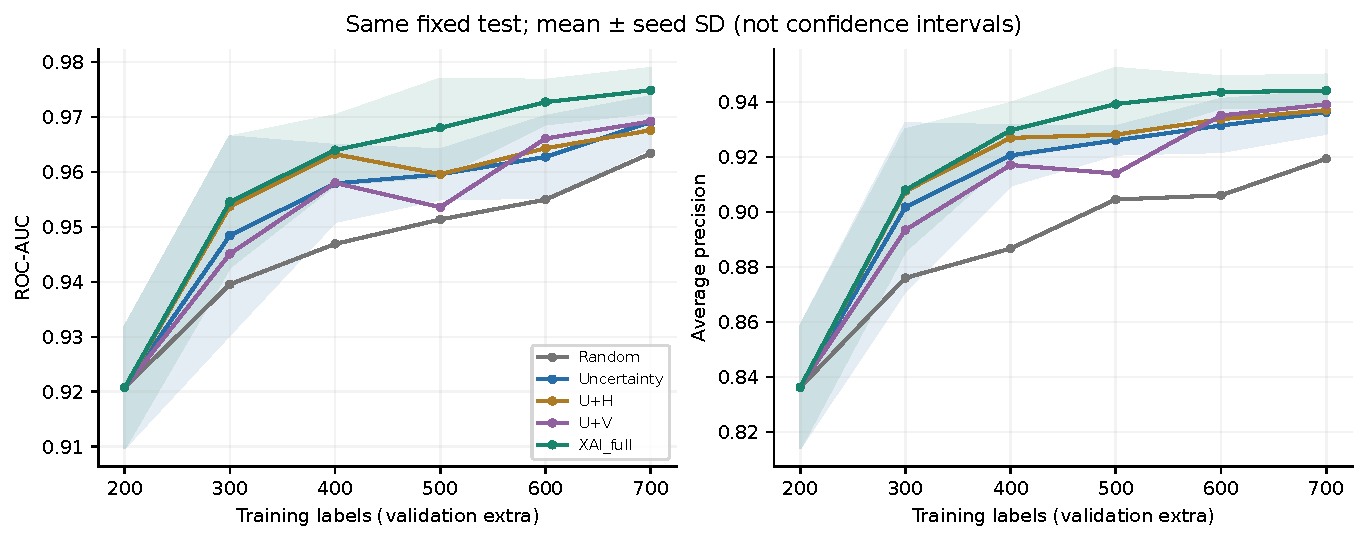
\includegraphics[width=\linewidth]{al_learning_curves.pdf}
\caption{Active-learning curves generated from the verified artifact. All methods
within a seed share the initial labeled set, split, and cumulative budget.}
\label{fig:learning-curves}
\end{figure}

\begin{figure}[t]
\centering
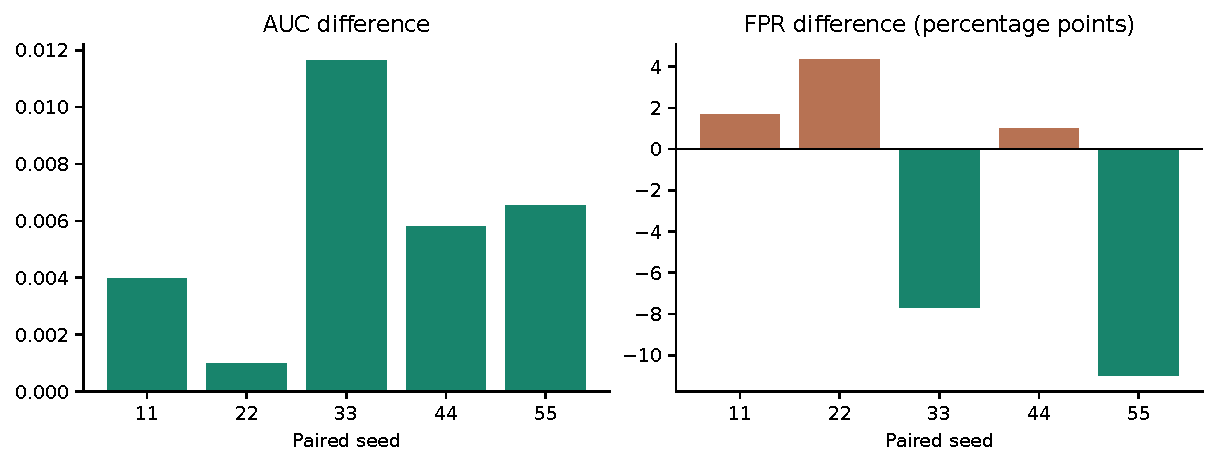
\includegraphics[width=\linewidth]{al_paired_differences.pdf}
\caption{Paired differences across seeds. AUC improvements are consistent for
$\xfull$ versus uncertainty, whereas FPR differences change sign.}
\label{fig:paired}
\end{figure}

Explanation-based acquisition incurred measurable scoring overhead. Mean total
query-scoring time across rounds was $0.1635$ s for $\xfull$, versus $0.0128$ s
for Uncertainty in the recorded two-thread environment. This approximately
13-fold ratio applies only to pool prediction, TreeSHAP, additivity checking, and
normalization in a small pilot. It excludes sorting, annotation, retraining, and
I/O and should not be interpreted as end-to-end operational latency.

The run trained 150 models: five seeds, five methods, and six budgets. The
maximum TreeSHAP additive reconstruction error in acquisition was
$4.44\times10^{-15}$. These checks reduce the likelihood that the observed
policy difference came from unequal initialization, accidental test access, or a
malformed attribution matrix. They do not resolve the external-validity limits of
the dataset.

\subsection{RQ2: Fidelity Under Controlled Deletion}

The separately fitted fidelity model obtained test ROC--AUC 0.980167 and AP
0.955338 before masking. Native TreeSHAP reconstructed the raw model score with
maximum absolute error $7.11\times10^{-15}$. Table~\ref{tab:fidelity} compares
sample-specific top-SHAP deletion with the mean across 20 equal-budget random
masks.

\begin{table*}[t]
\centering
\caption{Controlled feature-space deletion on one fixed model. Random AUC is the mean across 20 masks per $k$; bootstrap intervals condition on the fitted model.}
\label{tab:fidelity}
\scriptsize
\setlength{\tabcolsep}{3pt}
\begin{tabular}{ccccccc}
\toprule
$k$ & Original & Top-SHAP & Top-SHAP & 95\% bootstrap & Random & Random \\
 & AUC & AUC & drop & interval & AUC & drop \\
\midrule
10 & 0.980167 & 0.913933 & 0.066233 & [0.039044, 0.097026] & 0.979867 & 0.000300 \\
25 & 0.980167 & 0.818533 & 0.161633 & [0.122232, 0.207752] & 0.979910 & 0.000257 \\
50 & 0.980167 & 0.671200 & 0.308967 & [0.253428, 0.373968] & 0.979263 & 0.000903 \\
\bottomrule
\end{tabular}
\end{table*}

Deleting the top 10 coordinates reduced AUC by 0.0662, and increasing the budget
to 25 and 50 coordinates increased the drop to 0.1616 and 0.3090. Random deletion
had little effect on mean AUC at the same selected-coordinate counts. At $k=25$,
the top-SHAP drop was approximately $0.161633/0.0002567\approx630$ times the
mean random drop. This ratio is descriptive and sensitive to the near-zero
denominator; the absolute drops and intervals are the primary evidence.

Mean absolute probability change provides a second view. For top-SHAP masks it
was 0.1744, 0.2019, and 0.2123 at $k=10,25,50$, respectively. Random masks
produced mean changes of 0.00257, 0.00509, and 0.01018. The raw FF values for
top-SHAP deletion were 1.0394, 2.0045, and 2.1483. Values above one are possible
because (\ref{eq:ff}) normalizes by the original probability without clipping;
they are not percentages or bounded quality scores.

\begin{figure}[t]
\centering
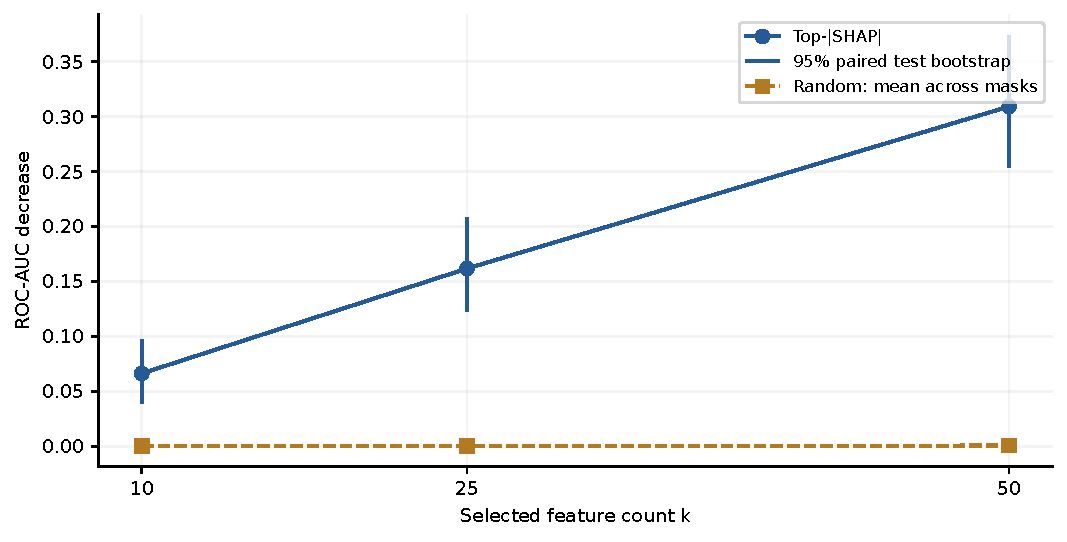
\includegraphics[width=\linewidth]{fidelity_deletion.pdf}
\caption{AUC under top-$|\mathrm{SHAP}|$ and random feature-space deletion. The
random control uses the same selected coordinate count.}
\label{fig:deletion}
\end{figure}

The explanation-geometry measures were EC=0.304373 and CF=0.587352. EC indicates
a modest positive association between pairwise similarity in standardized input
space and pairwise similarity in signed attribution space. It should not be read
as robustness to Gaussian noise or as a p-value based on 79,800 independent
pairs. CF indicates separation between positive- and negative-label SHAP
centroids relative to the largest per-sample attribution norm. It describes the
geometry of this fitted model and test set, not a causal boundary between malware
families.

Figure~\ref{fig:local-shap} provides a traceable local example from the fidelity
test set. Its role is illustrative: the aggregate conclusions come from all 400
test rows and controlled masks, not from selecting one visually persuasive case.

\begin{figure}[t]
\centering
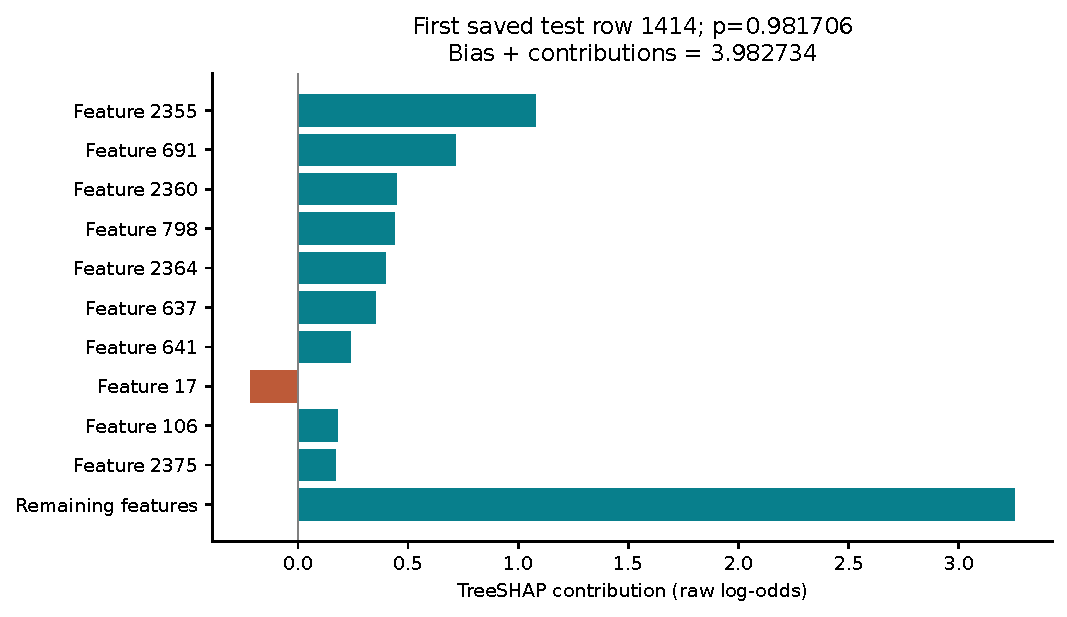
\includegraphics[width=\linewidth]{local_shap_example.pdf}
\caption{Traceable local TreeSHAP example generated from the fixed fidelity
model. Numeric coordinate labels reflect the available feature table.}
\label{fig:local-shap}
\end{figure}

RQ2 is therefore supported in a precise, limited sense: under replacement by
training-column means, coordinates ranked by absolute TreeSHAP have substantially
greater influence on the fitted model's ranking than uniformly selected
coordinates. The result does not establish that a masked vector corresponds to a
valid executable, that SHAP identifies causal ransomware behavior, or that the
same values hold for another trained model.

\subsection{RQ3: Status of PID Fusion}

The measured package records fusion as \texttt{not\_run} with the reason that real
dynamic reports aligned to validation and test IDs are required. The dynamic
template contains 800 row IDs and a schema for evidence collection, but its
provenance declares \texttt{signal\_origin=not\_collected}; it is not a result. No
synthetic score was substituted.

Consequently, this paper reports no PID AUC, AP, FPR, TPR, or latency. Values in
earlier thesis drafts cannot be traced to paired predictions under the locked
protocol and are excluded. This negative status is itself relevant to RQ3: a
valid claim requires the data lineage, ablations, state policy, and latency scope
specified in Sections~\ref{sec:problem}--\ref{sec:exp}. Until those inputs exist,
the framework contribution is the controller and evaluation design, not a
demonstrated improvement of the multi-stage system.
